% !TEX root = ../partial-blockchain.tex

The primary objective of this chapter is to increase the understanding of the Bitcoin through mathematical tools.

\section{Hash function}

Hash functions has been widely studied in computer science. In short, a hash function $h: \{0, 1\}^\infty \rightarrow \{0, 1\}^{n}$ has the following properties:

\begin{enumerate}
	\item $x = y \Rightarrow h(x) = h(y)$
	\item $h(x) \sim \mathcal{U}(0, 2^{n}-1)$, where $\mathcal{U}$ is the uniform distribution, i.e., $\forall a \in [0, 2^{n}-1], \mathbf{P}(h(x)=a) = \frac{1}{2^{n}}$
\end{enumerate}

In other words, when two inputs are the same, they have the same output. But, when the inputs are different, their outputs are uniformly distributed. Clearly, the hash functions are surjective but not injective. They are not injective because the image of $h$ has only $2^n$ elements and the domain has infinite elements. When $x \ne y$ and $h(x) = h(y)$, we say that $x$ and $y$ are a collision. A hash function is considered to be safe when it is unknown how to quickly find a collision of a given hash, i.e., one has to check all possible values until the correct one is found (known as the brute-force attack).

Bitcoin uses two hash functions: HASH-160 and HASH-256. The first has $n=160$ and consists of the composition of \textit{SHA-256} and \textit{RIPEMD-160}. The latter has $n=256$ and applies \textit{SHA-256} twice. The first is used in transactions' scripts and the latter in the mining algorithm. For both hash functions, it is infeasible to run a brute-force attack because it would demand, on average, either $2^{160}$ or $2^{256}$ trials, and those would take a tremendous amount of time even for the fastest known processors.

For further information about hash functions, see \citet{gilbert2003security, dobbertin1996ripemd}.


\section{Mining one block}

Let $\mathbb{B}$ be the set of Bitcoin blocks and $h: \mathbb{B} \rightarrow \{0, 1\}^{256}$ be the Bitcoin \textit{HASH-256} function. The mining process consists of finding $x \in \mathbb{B}$ such as $h(x) < A$, where $A$ is a given threshold. The smaller the $A$, the harder to find a new block. In fact, $\mathbf{P}(h(x) < A) = \frac{A}{2^{256}}$.

Hence, in order to find a new block, one must try different inputs ($x_1, x_2, \dots, x_k$) until they find a solution, i.e., all attempts will fail ($h(x_i) \geq A$ for $i < k$) but the last ($h(x_k) < A$). The probability of finding a solution exactly in the $k^{th}$ attempt follows a geometric distribution. Let $X$ be the number of attempts until a success, then $\mathbf{P}(X = k) = (1-p)^{k-1} p$, where $p = \frac{A}{2^{256}}$. Also, we have $\mathbf{P}(X \leq k) = 1 - (1-p)^k$. The average number of attempts is $\mathbf{E}(X) = 1/p$ and the variance is $\mathbf{V}(X) = \frac{1-p}{p^2}$.

In the Bitcoin's protocol, the given number $A$ is adjusted so that the network would find a new a block every 10 minutes, on average. Suppose that the Bitcoin's network is able to calculate $H$ hashes per second --- $H$ is the total hash rate of the network. The time required to find a solution would be $T=X/H$, and $\mathbf{E}(T) = \mathbf{E}(X)/H$ would be the average number of seconds to find a new block. So, the rule of finding a new block every 10 minutes ($\eta = 600$ seconds) --- on average --- leads to the following equation: $\mathbf{E}(T) = \eta = 600$. So, $\mathbf{E}(T) = \mathbf{E}(X)/H = \frac{1}{pH} = \eta = 600 \Rightarrow p = \frac{1}{\eta H}$. Finally, $\mathbf{E}(X) = \eta H$, $\mathbf{E}(T) = \eta$, $\mathbf{V}(X) = (\eta H)^2 - \eta H$, and $\mathbf{V}(T) = \eta^2 - \eta/H$.

The cumulative distribution function (CDF) of $T$ is $\mathbf{P}(T \leq t) = \mathbf{P}(X/H \leq t) = \mathbf{P}(X \leq tH) = 1 - (1-p)^{tH} = 1 - \left( 1-\frac{1}{\eta H} \right)^{tH}$. But, as the Bitcoin's network hash rate is really large, we may approximate the CDF of $T$ by $\lim_{H \rightarrow \infty} \mathbf{P}(T \leq t) = 1 - e^{-\frac{t}{\eta}}$, which is equal to the CDF of the exponential distribution with parameter $\lambda = \frac{1}{\eta}$.

\begin{theorem}
	When $H \rightarrow +\infty$, the time between blocks follows an exponential distribution with parameter $\lambda = \frac{1}{\eta}$, i.e., $\lim_{H \rightarrow +\infty} \mathbf{P}(T \leq t) = 1 - e^{-\frac{t}{\eta}}$.
\end{theorem}
\begin{proof}
\begin{align*}
	\mathbf{P}(T \leq t) &= 1 - (1-p)^{tH} \\
		     &= 1 - \left( 1 - \frac{1}{\eta H} \right)^{tH} \\
	\text{Replacing $u = \eta H$,} \\
	\lim_{H \rightarrow +\infty} \mathbf{P}(T \leq t) &= \lim_{u \rightarrow +\infty} 1 - \left( 1 - \frac{1}{u} \right)^{\frac{tu}{\eta}} \\
				&= \lim_{u \rightarrow +\infty} 1 - \left[ \left( 1 - \frac{1}{u} \right)^{u} \right]^{\frac{t}{\eta}} \\
				&= 1 - \left( 1/e \right)^{\frac{t}{\eta}} \\
				&= 1 - e^{-\frac{t}{\eta}}
\end{align*}
\end{proof}

Now, we would like to understand from which value of $H$ it is reasonable to assume that $T$ follows an exponential distribution.

\begin{theorem}
	$x > M \Rightarrow |(1+1/x)^x - e| < e/M$.
\end{theorem}
\begin{proof}
	Let's use the classical inequality $\frac{x}{1+x} < \log(1+x) < x$ for $x > -1$. So, $\frac{1/x}{1+1/x} < \log(1+x) < 1/x$. Simplifying, $\frac{1/x}{1+1/x} = 1/(1+x)$.  Thus, $1/(1+x) < \log(1+1/x) < 1/x \Rightarrow x/(1+x) < x \log(1 + 1/x) < 1$.

	As $\log(1 + \frac{1}{M}) > 0$ and $1 < 1 + \log(1 + \frac{1}{M})$.

	$x > M \Rightarrow 1/x < 1/M \Rightarrow 1+1/x < 1+1/M \Rightarrow 1/(1+1/x) > 1/(1+1/M) \Rightarrow x/(1+x) > M/(1+M)$.

	Again, $\log(1+x) < x \Rightarrow \log(1-1/M) < -1/M \Rightarrow 1 + \log(1-1/M) < (M-1)/M < M/(1+M)$, since $(x-1)/x < x/(x+1)$.

	Hence, $1 + \log(1-1/M) < M/(1+M) < x/(1+x) < x\log(1+1/x)$, and $x\log(1+1/x) < 1 < 1 + \log(1 + \frac{1}{M})$.

	Finally,

	\begin{align*}
		1 + \log(1-1/M) &< x\log(1+1/x) < 1 + \log(1 + \frac{1}{M}) \\
		e^{1 + \log(1-1/M)} &< e^{x\log(1+1/x)} < e^{1 + \log(1 + \frac{1}{M})} \\
		e \cdot e^{\log(1-1/M)} &< e^{\log((1+1/x)^x)} < e \cdot e^{\log(1 + \frac{1}{M})} \\
		e(1-1/M) &< (1+1/x)^x < e(1 + \frac{1}{M}) \\
		e-e/M &< (1+1/x)^x < e + e/M \\
		-e/M &< (1+1/x)^x - e < e/M \\
	\end{align*}
	Therefore, $\left| \left( 1+1/x \right)^x - e \right| < e/M$.
\end{proof}

We may consider $H$ big enough to say that $T$ follows an exponential distribution when $e/H < \epsilon$, where $\epsilon$ is the maximum approximation error. When $\epsilon = 10^{-6} \Rightarrow H > e \cdot 10^6$. So, when $H > 2.6 \text{Mh/s}$, our approximation is good enough.

The symmetrical confidence interval with level $\alpha$ would be $[t_0, t_1]$, where $\mathbf{P}(t_0 < T < t_1) = 1-\alpha$, $\mathbf{P}(T<t_0) = \alpha/2$, and $\mathbf{P}(T>t_1) = \alpha/2$. These conditions give the following equations: $1 - e^{-t_0/\eta} = \alpha/2$, and $e^{-t_1/\eta} = \alpha/2$. Solving these equations, we have $t_0 = -\eta \ln{(1 - \alpha/2)}$, and $t_1 = -\eta \ln{(\alpha/2)}$.

For instance, if $\alpha = 10\%$, then $t_0 = 30.77$ and $t_1 = 1797.44$ (or $[0.51, 30.76]$ in minutes). Thus, 90\% of the time the intervals between blocks are between 30 seconds and 30 minutes, with average of 10 minutes.

The fact that the time between blocks follows an exponential distribution with $\lambda = 1/\eta = pH$ may be used to estimate the total network's hash rate (or a miner's hash rate). For further information, see \cite{ozisikestimation}.


\section{Mining several blocks}

Let $T_1, T_2, T_3, \dots, T_n$ be the time to find the first block ($T_1$), then the time to find the second block ($T_2$), and so on. Let's analyze the distribution of $Y_n = \sum_{i=1}^{n} T_i$ which is the total time to find the next $n$ blocks. As $Y_n$ is the sum of random variables which follow an exponential distribution with same $\lambda = \frac{1}{\eta}$, then $Y_n \sim \text{Erlang}(n, \frac{1}{\eta})$. Thus, the CDF of $Y$ would be $\mathbf{P}(Y_n < t) = 1 - \sum_{k=0}^{n-1} \frac{1}{k!} e^{-\lambda t} (\lambda t)^k$.

Many exchanges require at least six confirmations in order to accept a deposit in Bitcoin. So, for $n=6$, $\mathbf{P}(Y_6 < 1 \text{ hour}) = \mathbf{P}(Y_6 < 3600) = 0.5543$, i.e., only 55\% of the deposits will be accepted in one hour. The symmetrical confidence interval with $\alpha=10\%$ is $[27, 105]$ in minutes. Thus, 90\% of the times, it will take between 27 minutes and 1 hour and 45 minutes to have your deposit accepted --- assuming that your transaction will be confirmed in the very next block. The pdf of $Y_6$ is shown in Figure \ref{fig-bitcoin-time-6-blocks}, in which the 10\% symmetrical confidence interval is shown in the white area. The average total time of six confirmations is $\mathbf{E}(Y_6) = 6 \cdot 600 = 3600 = 60 \text{ minutes}$.

\begin{figure}[ht]
\centering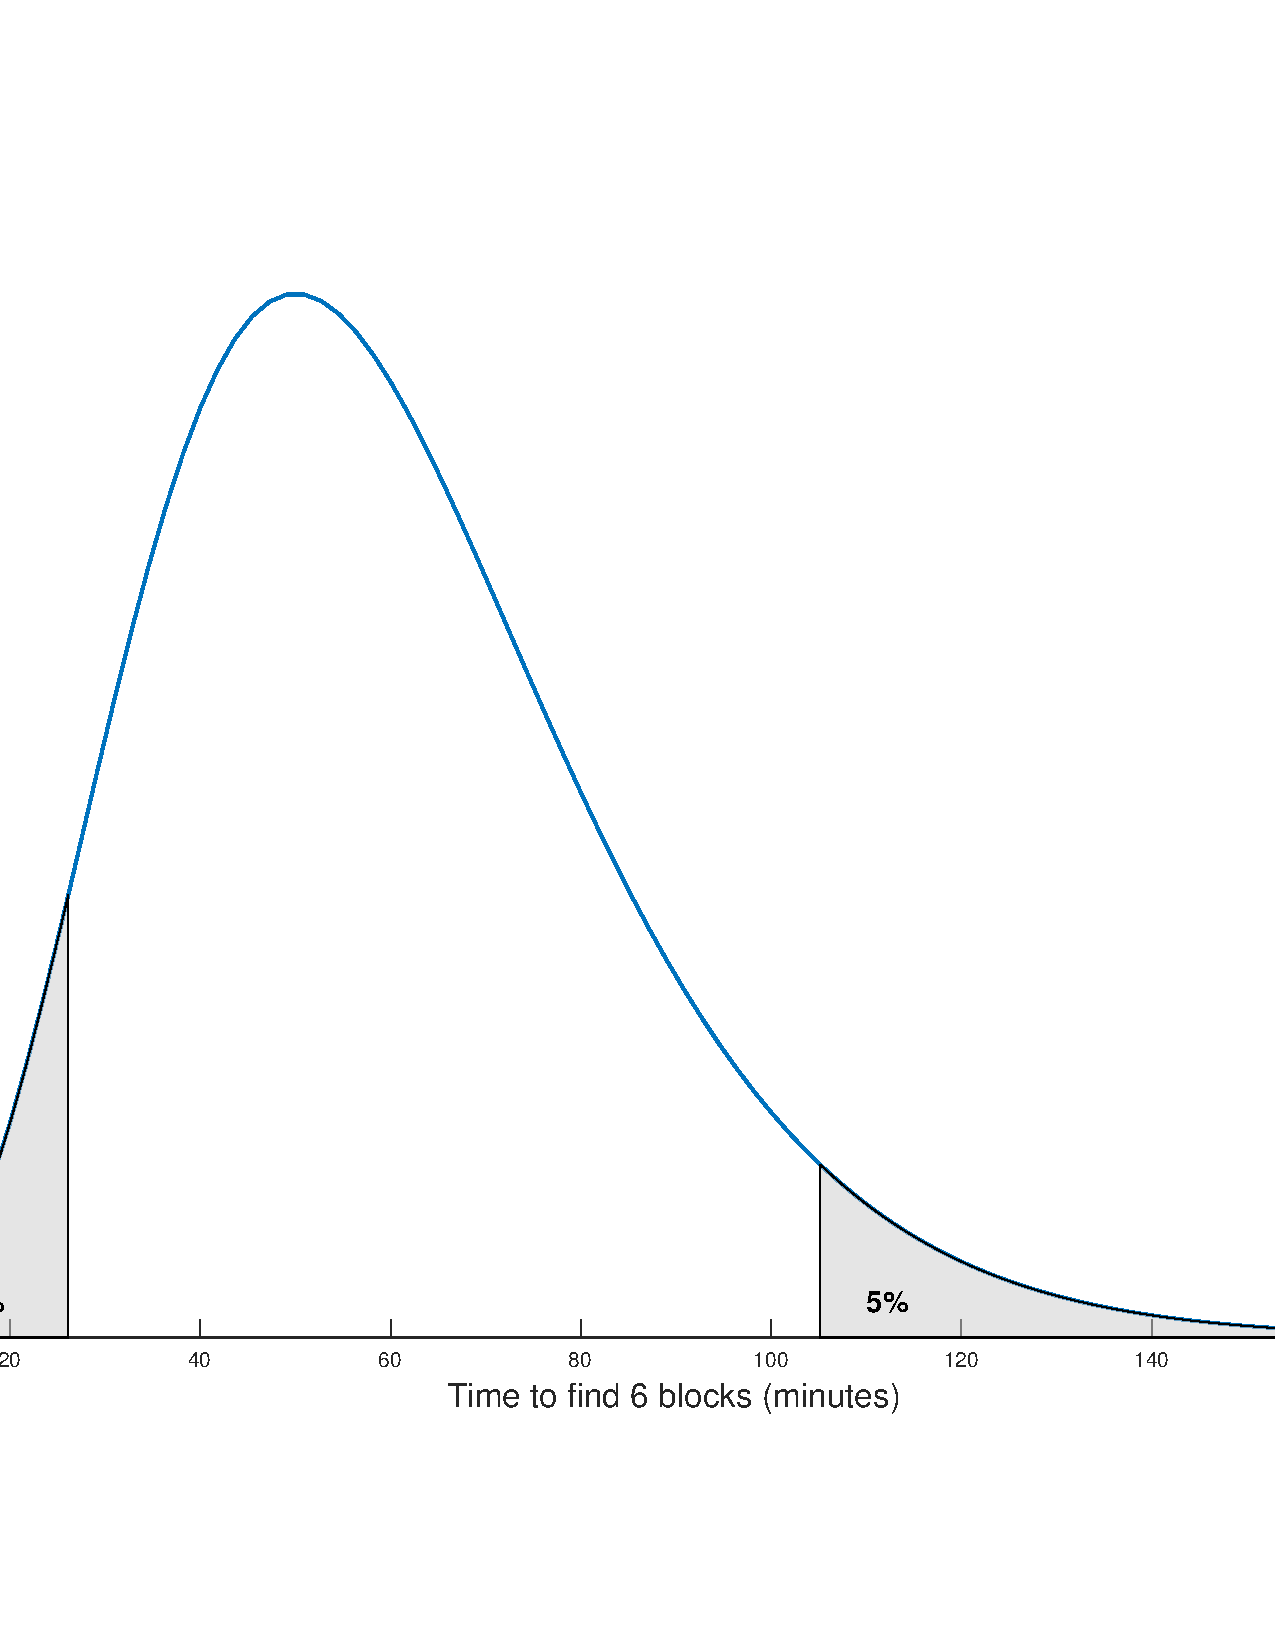
\includegraphics[width=\textwidth]{./images01/time-6-blocks.pdf}
\caption{Probability density function of $Y_6$, i.e., probability of finding 6 blocks after time $t$. The shaded areas shows the lower 5\% and upper 5\% of the pdf.\label{fig-bitcoin-time-6-blocks}}
\end{figure}

\section{Mining for a miner}

Let's analyze the probability of finding a new block for a miner who has $\alpha$ percent of the network's total hash rate. Let $T_\alpha = \frac{X}{\alpha H}$ be the time required for the miner to find a new block. As $T_\alpha = \left( \frac{1}{\alpha} \right) T$, when $H \rightarrow +\infty$, $T_\alpha$ also follows an exponential with parameter $\lambda_\alpha = \frac{\alpha}{\eta}$. Hence, we confirm the intuition that the miner with $\alpha$ percent of the network's total hash power will find $\alpha$ percent of the blocks.

\begin{theorem}
	When the miner with $\alpha$ percent of the network's total hash rate is part of the mining network, $\mathbf{P}(\text{next block is from $T_\alpha$}) = \alpha.$
\end{theorem}
\begin{proof}
\begin{align*}
	\mathbf{P}(\text{next block is from $T_\alpha$}) &= P \left( T_\alpha = \min\{T_\alpha, T_{1-\alpha}\} \right) \\
		&= \frac{\lambda_\alpha}{\lambda_\alpha + \lambda_{1-\alpha}} \\
		&= \frac{\alpha/\eta}{\alpha/\eta + (1-\alpha)/\eta} \\
		&= \frac{\alpha}{\alpha + 1 - \alpha} \\
		&= \alpha.
\end{align*}
\end{proof}

\begin{theorem}
	When one miner with $\alpha$ percent of the network's total hash rate multiplies their hash rate by $m$, the probability of this miner find the next block is multiplied by $\frac{m}{m \alpha + 1 - \alpha}$.
	\label{thm-miner-multiply}
\end{theorem}
\begin{proof}
	When miners increase their hash rate, they also increase the network's total hash rate. Let $H$ be the network's hash rate before the increase. Thus, the network's total hash rate after the increase is $H + (m-1) \alpha H = (1 - \alpha + m \alpha) H$. So,
\begin{align*}
	\mathbf{P}(\text{next block is from $T_{m \alpha}$}) &= P \left( T_{m \alpha} = \min\{T_{m \alpha}, T_{1-\alpha}\} \right) \\
		&= \frac{\lambda_{m \alpha}}{\lambda_{m \alpha} + \lambda_{1-\alpha}} \\
		&= \frac{m \alpha/\eta}{m \alpha/\eta + (1-\alpha)/\eta} \\
		&= \frac{m \alpha}{m \alpha + 1-\alpha} \\
		&= \alpha \left( \frac{m}{m \alpha + 1 - \alpha} \right).
\end{align*}
\end{proof}

\begin{cor}
	If one miner has a really tiny percent of the network's total hash rate, then multiplying their hash rate by $m$ approximately multiplies their probability of finding the next block by $m$.
\end{cor}
\begin{proof}
	$$\lim_{\alpha \rightarrow 0} \mathbf{P}(\text{next block is from $T_{m \alpha}$}) = \lim_{\alpha \rightarrow 0} \frac{m}{m \alpha + 1 - \alpha} = m.$$
\end{proof}

That way, it is not exactly correct to say that when one doubles their hash rate, their probability will double as well. It is only true for small miners.


\section{Orphan blocks}
% Probabilidade de orfão
An orphan block would be created if a new block is found during the propagation time of a new block. Let $\alpha$ be the percentage of the total hash rate of the node which is outdated, and $\Delta t$ the propagation time in seconds. Thus, $\mathbf{P}(\text{new orphan}) = \mathbf{P}(T < \Delta t) = 1 - e^{-\frac{\alpha \Delta t}{\eta}}$.

Bitcoin peer-to-peer network is a gossip network, where miners are semi-randomly connected to each other, and each miner sends all information it receives to all its peers. According to \citet{decker2013information}, the average time for a new block propagate over the network is 12.6 seconds, while the 95\% percentile is 40 seconds, which indicates a long-tail distribution. \citet{bitcoinstats} has measured the propagation time between 2013 and 2017. During 2017, the worst daily 90\% percentile was 21 seconds. Notice that both results may not be contradictory because Bitcoin network is continuously evolving.

For instance, if a node has 10\% of the total hash rate and it takes 30 seconds to receive the update, then $\mathbf{P}(\text{new orphan}) = 1 - e^{-\frac{0.1 \cdot 30}{600}} = 0.004987$, which is almost 0.5\%. I would say that a node with 10\% of the total hash rate would be well connected and it would take less time to receive the update, so, the probability would be even smaller than 0.5\%.

Another important factor is that, as Bitcoin is open-source, miners are free to change the gossip algorithm, which leads to the network incentives. See \citet{babaioff2012bitcoin} for an analysis of the incentives to miners forward new blocks and transactions in the network.

For further information about gossip algorithms, see \citet{shah2009gossip}.


\section{Analysis of network's hash rate change}
% Análise: Mudança no network's hash rate antes de atualizar o $A$.

The difficulty, given by the number $A$, is adjusted every 2016 blocks. As, $\mathbf{P}(13 \text{ days} < Y_{2016} < 15 \text{ days}) = \mathbf{P}(13 \cdot 24 \cdot 3600 < Y_{2016} < 14 \cdot 24 \cdot 3600) = 0.9986$, it is expected that the total time to find 2016 blocks will be between 13 and 15 days, assuming that the network's hash rate remains constant. If it takes less than the expected time, it means that the network's total hash rate has increased. While if it takes more than the expected time, it means that the network's total hash rate has decreased. So, let's analyze what happens when the network's hash rate changes significantly.

%Let's assume that the network's total hash rate will change only once, from $H$ to $\alpha H$ --- so, if $\alpha = 1$, there would be no change, if $\alpha > 1$, there would be an increase, and if $\alpha < 1$, there would be a decrease. As the time required to find a new block would be $T_\alpha = \frac{X}{\alpha H}$, we got the same random variable as we have gotten when analyzing a miner with $\alpha$ percent of the network's total hash rate. But, the analysis will be different because here $\alpha$ may be greater than one.

Let $H \cdot u(t)$ be the network's total hash rate over time. So, the number of hashes calculated in $t$ seconds is $H \int_0^t u(t) dt$. Hence, $\mathbf{P}(T \leq t) = \mathbf{P}(X \leq H \int_0^t u(t)dt)$. When $H \rightarrow +\infty$, $\mathbf{P}(T \leq t) = 1 - e^{-\frac{1}{\eta} \int_0^t u(t) dt}$, and the pdf of $T$ is $\frac{u(t)}{\eta} \cdot e^{-\frac{1}{\eta} \int_0^t u(t)dt}$.

\subsection{Hash rate suddenly changing}

Let's say that the network's total hash rate has suddenly multiplied by $\alpha$. So, $u(t) = \alpha$, $\int_0^t u(t) dt = \alpha t$, and $T$ also follows an exponential distribution, but with $\lambda = \frac{\alpha}{\eta}$. Thus, $Y_n^\alpha = \sum_{i=1}^{n} T_i^\alpha \sim \text{Erlang}(n, \frac{\alpha}{\eta})$. Thus, $\mathbf{E}[Y_{n}^\alpha] = \frac{\mathbf{E}[Y_{n}]}{\alpha}$, i.e., the average total time required to find $n$ blocks will be divided by $\alpha$, while $\mathbf{V}[Y_{n}^\alpha] = \frac{\mathbf{V}[Y_n]}{\alpha^2}$ and the variance will be divided by $\alpha^2$. Hence, on one hand, when the network's hash rate increases ($\alpha > 1$), the 2016 blocks will be found earlier. On the other hand, when the network's hash rate decreases ($\alpha < 1$), the 2016 blocks will be found later.

For example, if the network's total hash rate suddenly doubles ($\alpha = 2$), then $\mathbf{P}(6.5 \text{ days} < Y_{2016} < 7.5 \text{ days}) = 0.9986$, and the time required to find 2016 blocks halved. On the other side, if the network's total hash rate suddenly halves ($\alpha = 0.5$), then $\mathbf{P}(27 \text{ days} < Y_{2016} < 29 \text{ days}) = 0.9469$, and the time required to find 2016 blocks doubled. It is an important conclusion, since it shows that even if half of the network stops mining, it will only double the time to the next difficulty adjustment, i.e., the time between blocks will be 20 minutes for, at most, the next 29 days, at which point the adjustment will occur and everything will be back to the normal 10 minutes between blocks.

% TODO Step-wise analysis

\subsection{Hash rate smoothly changing}

Let $u(t) = \frac{1+abx}{1+bx}$. It is an useful function because $u(0) = 1$ and $\lim_{t \rightarrow \infty} u(t) = a$. The bigger the $b$, the faster $u(t) \rightarrow a$. For example, if $a=2$, it means $H$ would be smoothly doubling. If $a=0.5$, it means $H$ would be smoothly halving.

It is easy to integrate $u(t)$ because $\frac{1+abx}{1+bx} = \frac{1-a}{1+bx} + a$, which yields $\int_0^t u(x) dx = at + \frac{1-a}{b} \log(1+bt)$. So,
$$F_T(t) = 1 - (1+bt)^{\frac{\lambda(a-1)}{b}} e^{-\lambda at}.$$
$$f_T(t) = \lambda \left( \frac{1+abt}{1+bt} \right) (1+bt)^{\frac{\lambda(a-1)}{b}} e^{-\lambda at}.$$

Assuming that $n = \frac{\lambda(a-1)}{b}$ is integer, we have:
$$F_T(t) = 1 - (1+bt)^n e^{-\lambda at}$$

Let $\mathcal{L}$ be the Laplace Transform. Thus,
\begin{align*}
\mathcal{L}\{F_T(t)\} &= \mathcal{L}\{1 - (1+bt)^n e^{-\lambda at}\} \\
	&= \mathcal{L}\{1\} - \mathcal{L}\{(1+bt)^n e^{-\lambda at}\} \tag{$\mathcal{L}$ is a linear operator} \\
	&= \frac{1}{s} - \mathcal{L}\{(1+bt)^n e^{-\lambda at}\} \\
	&= \frac{1}{s} - \sum_{k=0}^n \binom{n}{k} b^k \mathcal{L}\{t^k e^{-\lambda at}\} \\
	&= \frac{1}{s} - \sum_{k=0}^n \binom{n}{k} b^k \frac{k!}{(s+\lambda a)^{k+1}}
\end{align*}

Hence, as $\mathcal{L}\{f_T(t)\} = s \mathcal{L}\{F_T(t)\}$,

$$\mathcal{L}\{f_T(t)\} = 1 - \sum_{k=0}^n \binom{n}{k} \frac{s b^k k!}{(s+\lambda a)^{k+1}}$$

Then,

\begin{align*}
\frac{d}{ds} \mathcal{L}\{f_T(t)\}
	&= - \sum_{k=0}^n \binom{n}{k} b^k k! \frac{d}{ds} \frac{s}{(s+\lambda a)^{k+1}} \\
	&= - \sum_{k=0}^n \binom{n}{k} b^k k! \left[ \frac{1}{(s+a\lambda)^{k+1}} - \frac{s(k+1)}{(s+a \lambda)^{k+1}} \right] \\
\frac{d}{ds} \mathcal{L}\{f_T(t)\}|_{s=0}
	&= - \sum_{k=0}^n \binom{n}{k} b^k k! \frac{1}{(\lambda a)^{k+1}} \\
	&= - \frac{1}{a\lambda} \sum_{k=0}^n \binom{n}{k} k! \left( \frac{b}{\lambda a} \right)^k \\
	&= - \frac{1}{a\lambda} \sum_{k=0}^n \frac{n!}{(n-k)!} \left( \frac{b}{\lambda a} \right)^k \\
	&= - \frac{1}{a\lambda} \left[ n! \sum_{k=0}^n \frac{1}{(n-k)!} \left( \frac{b}{\lambda a} \right)^k \right] \\
	&= - \frac{1}{a\lambda} \left[ n! \sum_{k=0}^n \frac{1}{k!} \left( \frac{b}{\lambda a} \right)^{n-k} \right] \tag{$k \rightarrow n-k$} \\
	&= - \frac{1}{a\lambda} \left[ n! \left(\frac{b}{\lambda a}\right)^n \sum_{k=0}^n \frac{1}{k!} \left( \frac{b}{\lambda a} \right)^{-k} \right] \\
	&= - \frac{1}{a\lambda} \left[ n! \left(\frac{b}{\lambda a}\right)^n \sum_{k=0}^n \frac{1}{k!} \left( \frac{\lambda a}{b} \right)^{k} \right]
\end{align*}

Finally, as $\mathbf{E}[T] = -\mathcal{L}\{f_T(t)\}|_{s=0}$,
$$\mathbf{E}[T] = \frac{1}{\lambda a} \left[ n! \left(\frac{b}{\lambda a}\right)^n \sum_{k=0}^n \frac{1}{k!} \left( \frac{\lambda a}{b} \right)^{k} \right] \text{, where $n = \frac{\lambda(a-1)}{b}$}$$

Let's check this equation for already known scenarios. When $a=1$, then $n=0$ and $\mathbf{E}[T] = 1/\lambda$. When $b \rightarrow +\infty$, it reduces to the case in which the hash rate is multiplied by $a$, which we have already studied. In fact, $b \rightarrow +\infty$ yields $n \rightarrow 0$, $u(t) \rightarrow a$, and $\mathbf{E}[T] = \frac{1}{\lambda a}$.

\begin{theorem}
	$$a > 1 \text{ and } x > M \Rightarrow \left| \frac{1+abx}{1+bx} - a \right| < \frac{a-1}{1+bM}$$
\end{theorem}
\begin{proof}
$x > M \Rightarrow \frac{1}{1+bx} < \frac{1}{1+bM}$. As $1-a<0$, $\frac{1-a}{1+bx} > \frac{1-a}{1+bM}$. Thus, $\frac{1-a}{1+bM} < \frac{1-a}{1+bx} + a - a = \frac{1+abx}{1+bx} - a < 0 < \frac{a-1}{1+bM}$. Hence, $-\frac{a-1}{1+bM} < \frac{1+abx}{1+bx} - a < \frac{a-1}{1+bM}$.
\end{proof}

For instance, if we would like to know the impact of smoothly double the hash rate in the next week, then the parameters would be $\lambda = 1/600$, $a=2$, $M=1\text{ week}=3600\cdot24\cdot7 = 604,800$, $b$ can be calculated using $\epsilon = \frac{a-1}{1+bM} < 0.01$, which yields $b > 0.000163690$ and $n < 10.1818$. So, for $n=10$, then $b=0.000166666$ and $\epsilon = 0.009823 < 0.01$, as expected. Finally, $\mathbf{E}[T] = 557.65$. In other words, during the next week, the average time between blocks will be 9 minutes and 17 seconds, instead of the normal 10 minutes. If the hash rate had suddenly doubled, the average time between blocks would be 5 minutes.

%$$\mathbf{E}[T] = -\mathcal{L}\{f_T(t)\}|_{s=0} = \frac{b^n n! 600^{n+1}}{a^{n+1}} e^{\frac{a}{600b}} \text{, where $n = \frac{a-1}{600b}$}$$


%$a > 1, x > M \Rightarrow 1 + bx > 1 + bM \Rightarrow \frac{1}{1+bx} < \frac{1}{1+bM} \Rightarrow \frac{1-a}{1+bx} + a > \frac{1-a}{1+bM} + a \Rightarrow \frac{1+abx}{1+bx} - a > \frac{1-a}{1+bM}$.


\subsection{Piecewise linear model of hash rate change}

Let's analyze what would happen if the network's hash rate is growing linearly with angular coefficient $a^2$, i.e., $u(a, b, t) = a^2t + b$. Thus, $\mathbf{P}(T \leq t) = 1 - e^{-\frac{bt + a^2t^2/2}{\eta}}$.

It is well known that $\mathbf{E}(T) = \int_{0}^{\infty} 1 - \mathbf{P}(T \leq t) dt$. Thus, replacing $y = \frac{a^2 t + b}{a \sqrt{2 \eta}}$, and using the fact that $\int_0^\infty e^{-x^2} dx = \frac{\sqrt{\pi}}{2} \erf(x)$, we have:

\begin{align}
\mathbf{E}(T)|_{t_1}^{t_2} &= \int_{t_1}^{t_2} \exp \left( - \frac{bt + a^2 t^2/2}{\eta} \right) dt \nonumber \\
	&= \frac{\sqrt{2 \eta}}{a} \exp \left( \frac{b^2}{2a^2 \eta} \right) \int_{y_1}^{y_2}  \exp(-y^2) dy \nonumber \\
	&= \frac{\sqrt{2 \eta}}{a} \exp \left( \frac{b^2}{2a^2 \eta} \right) \frac{\sqrt{\pi}}{2} [\erf(y_1) - \erf(y_2)] \nonumber \\
	&= \frac{\sqrt{2 \pi \eta}}{2a} \exp \left( \frac{b^2}{2a^2 \eta} \right) \left[\erf(y_2) - \erf(y_1) \right]
\end{align}

Where $y_1 = \frac{a^2 t_1 + b}{a \sqrt{2 \eta}}$ and $y_2 = \frac{a^2 t_2 + b}{a \sqrt{2 \eta}}$.

Thus, $\mathbf{E}(T) = \mathbf{E}(T)|_0^\infty$. When $t_1 = 0 \Rightarrow y_1 = \frac{b^2}{2 \sqrt{2 \eta}}$ and $t_2 \rightarrow \infty \Rightarrow y_2 \rightarrow \infty \Rightarrow \erf(y_2) = 1$, then:

$$
\mathbf{E}(T) = \frac{\sqrt{2 \pi \eta}}{2a} \exp \left( \frac{b^2}{2a^2 \eta} \right) \left[1 - \erf\left(\frac{1}{a \sqrt{2 \eta}}\right)\right]
$$


\subsection{Comparison of the models}

In order to compare the hash rate change models, namely (i) suddenly change, (ii) smoothly change, and (iii) linear change, I have applied each of them to the same scenarios. In the first scenario, the hashrate will double in the next week, whereas, in the second scenario, it will halve in the next week.

In both the smoothly change model and the linear change model, I could have calculated the average time between blocks during the whole week. It would not give us much information, because the time between models would be increasing (or reducing) more and more as the days goes by. And we are really interested in the average time between blocks throughout the days, and not the average of the whole week.

Thus, I have analyzed a piecewise hash rate change, i.e., I have calculated the average time between blocks for each hour throughout the week. First, I split the whole week into $24 \cdot 7$ intervals, $(t_0, t_1, t_2, \dots, t_168)$, where $t_i = 3600i$. Then, I calculated the average for each interval $(t_k, t_{k+1})$. Let $H_k^0$ and $H_k^1$ be the initial and final hash rate of the $(t_k, t_{k+1})$ interval. So, I also ensured the continuity of the hash rate between consecutive intervals, i.e., $H_k^1 = H_{k+1}^0$.

I compared both the smoothly change model and the linear change model with the suddenly change model. The difference between them is negligible. Let $\epsilon$ be the maximum absolute error between the models, than $\epsilon < 0.8$ and $\epsilon/H < 0.2\%$, for all intervals. The maximum absolute error between the linear and the suddenly change models can be seen in Figure \ref{fig:bitcoin-H-change-error}.

\begin{figure}[!htb]
\centering 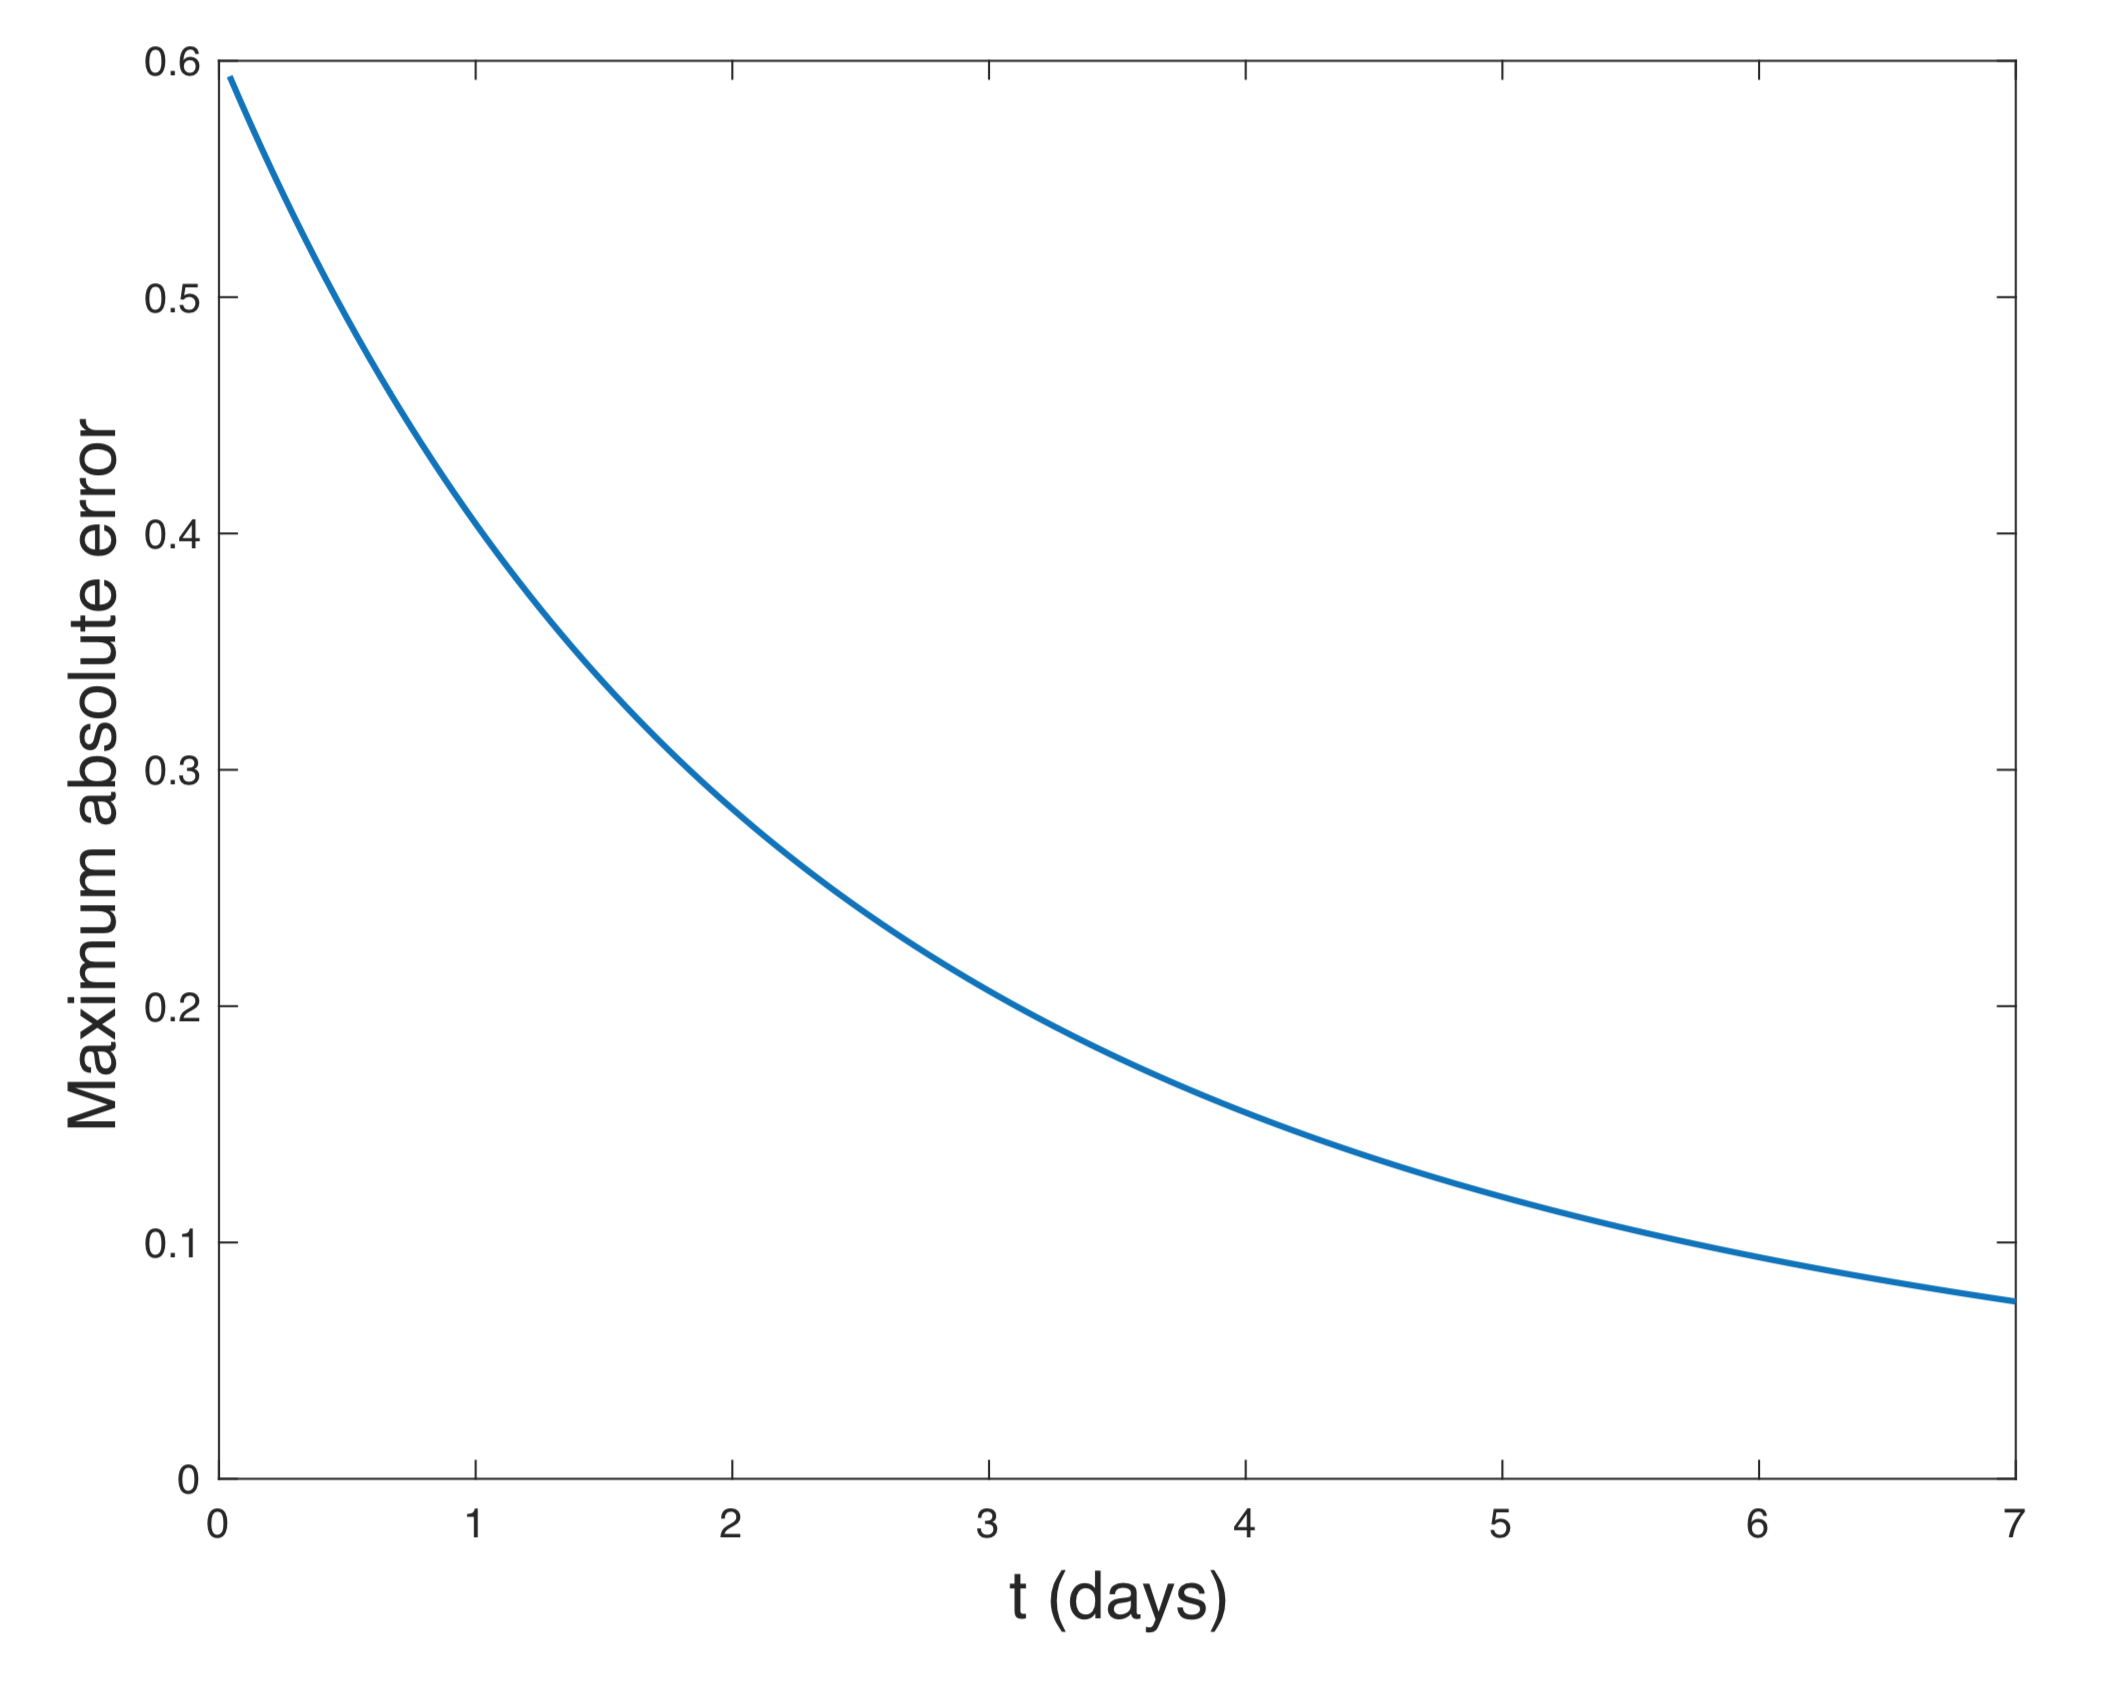
\includegraphics[width=0.7\textwidth]{./images01/H-max-abs-error.png}

\caption{Maximum absolute error between the linear and the suddently change models. \label{fig:bitcoin-H-change-error}}
\end{figure}

Therefore, we may conclude that it is reasonable to approximate the average time between blocks using only the suddenly change model in each interval of one hour.

The average time between blocks throughout the days can be seen in Figure \ref{fig:bitcoin-H-change}. It was calculated using the suddenly change model with the hash rate changing linearly during the week.

\begin{figure}[!htb]
\centering
\subfloat[Doubling the hash rate]{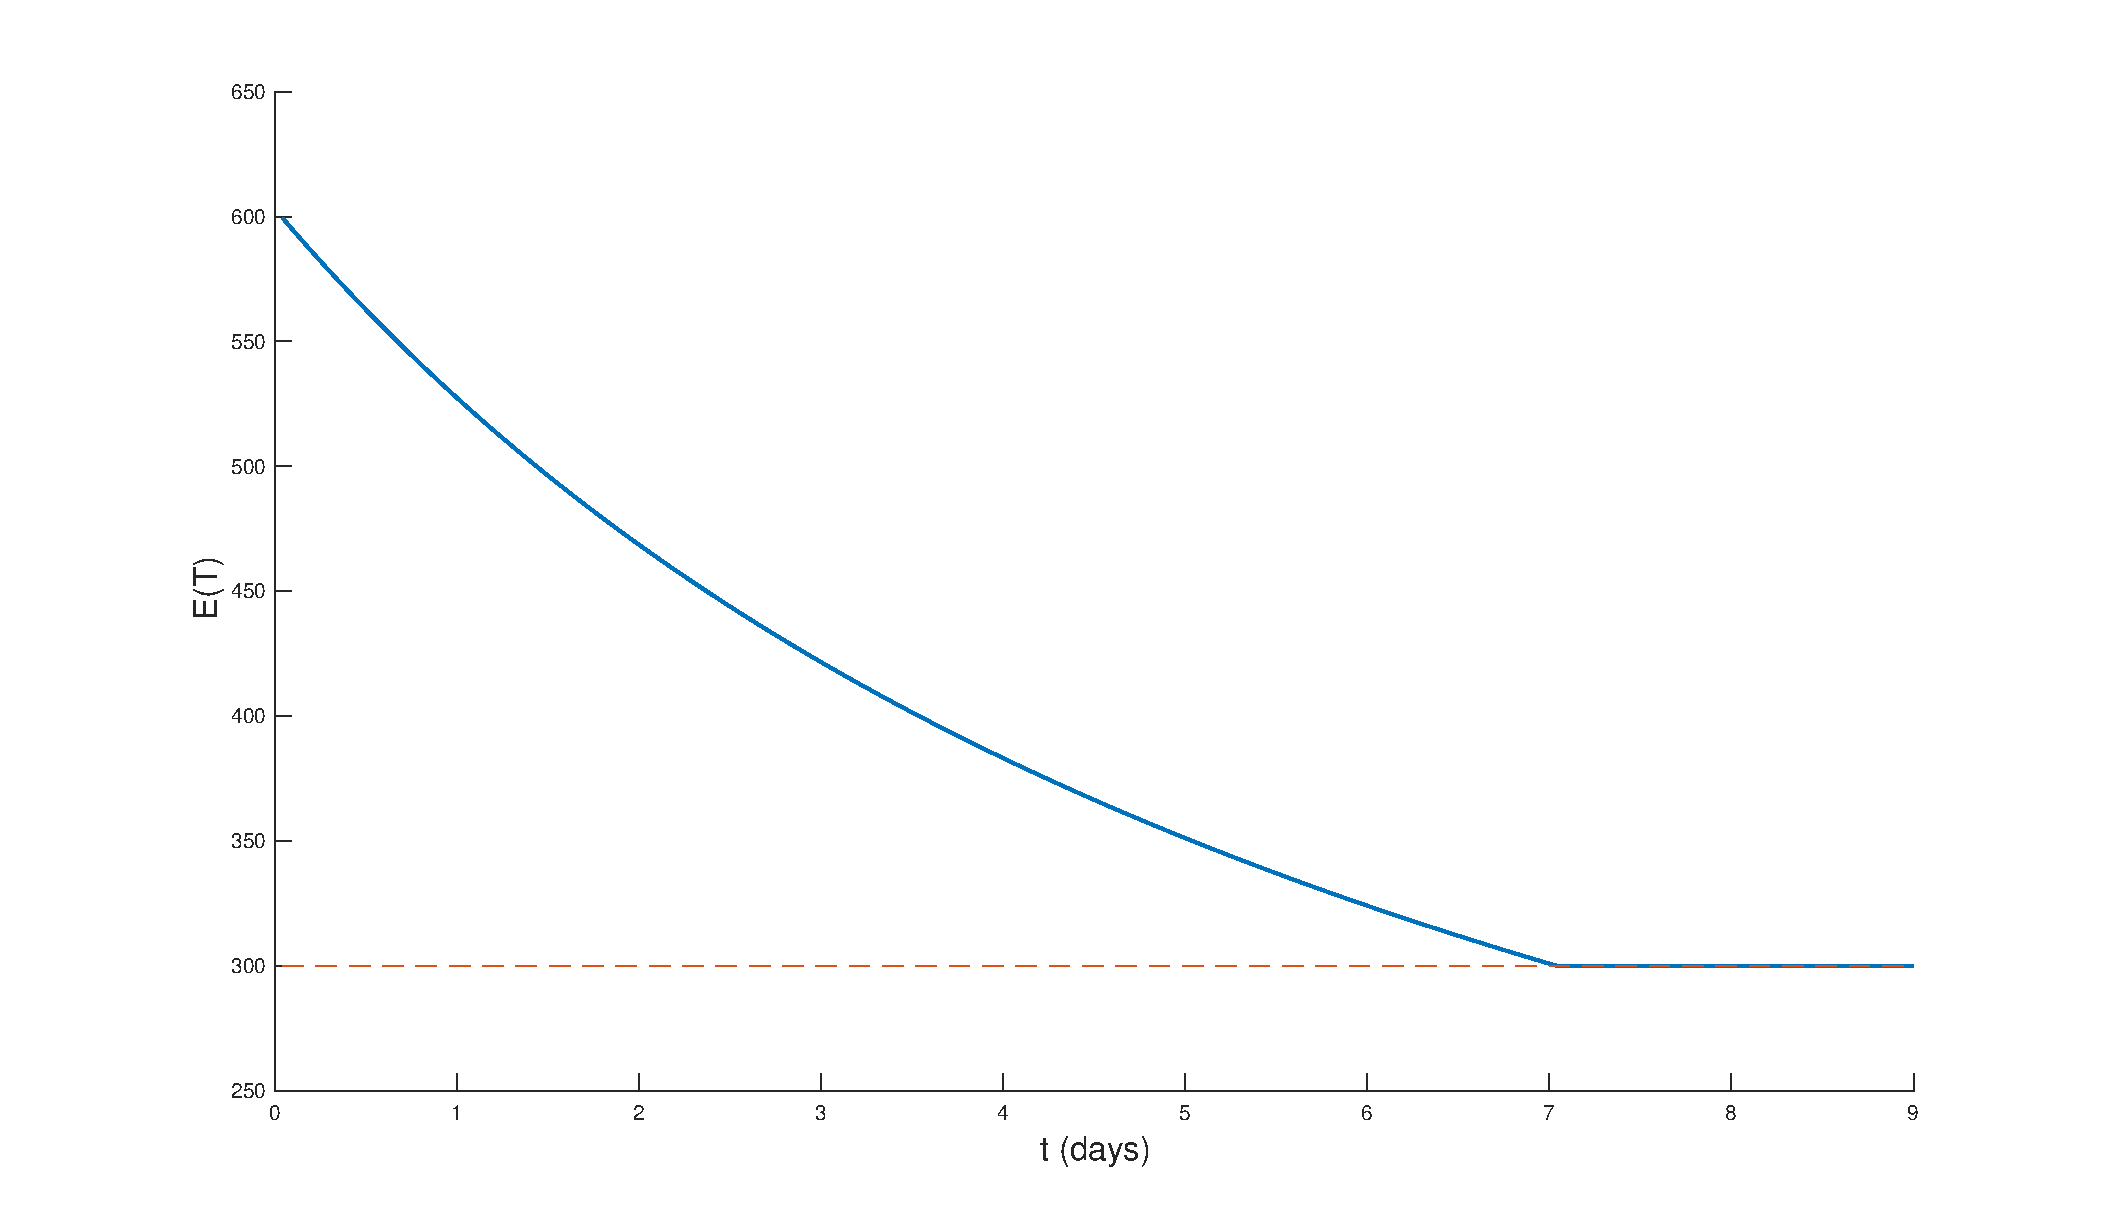
\includegraphics[width=\textwidth]{./images01/H-double-week.pdf}}

\subfloat[Halving the hash rate]{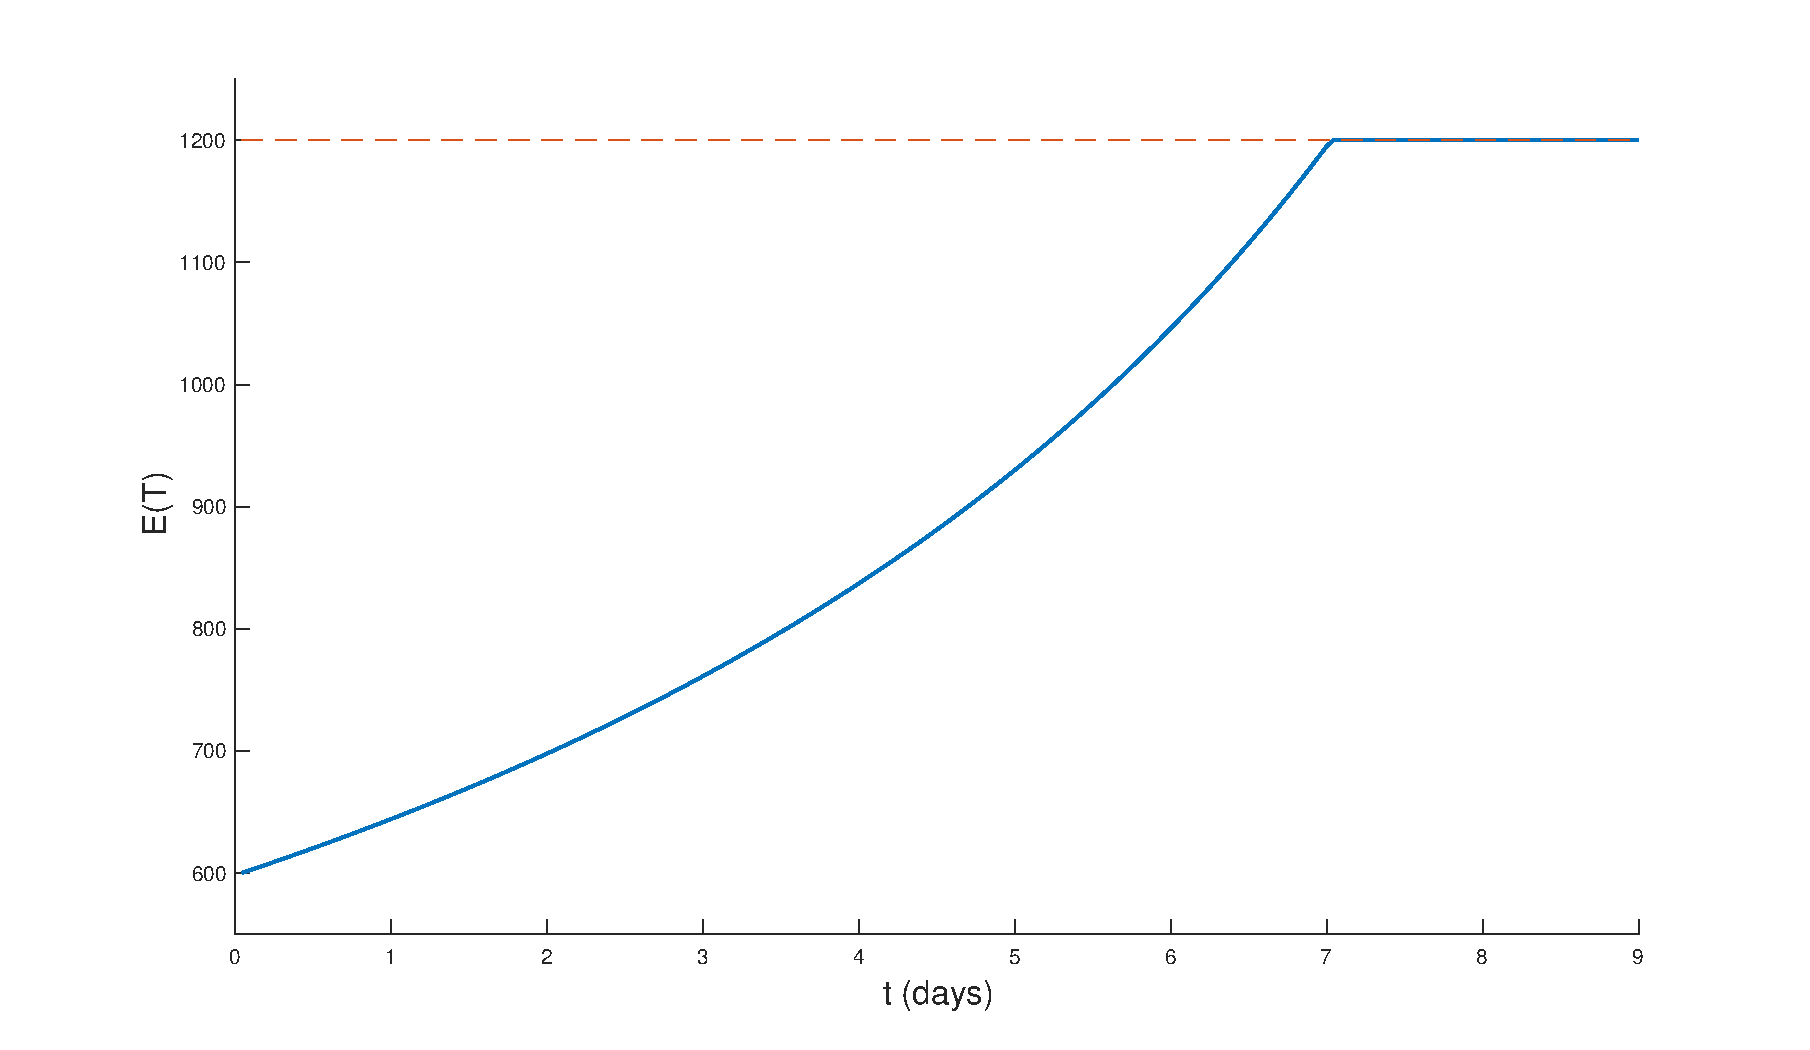
\includegraphics[width=\textwidth]{./images01/H-halves-week.pdf}}

\caption{The average time between blocks when the hash rate changes over time. \label{fig:bitcoin-H-change}}
\end{figure}

%In order to obtain $\mathbf{E}(T)$, we will use the formula $\frac{d}{ds}T^*(s)|_{s=0} = -\mathbf{E}(T)$, where $T^*$ is the Laplace transform of the pdf of T.
%
%Let $f_T(x)$ be the pdf of T and $F_T(x)$ be the cdf of T, i.e., $F_T(x) = \int_0^x f_T(t) dt$. Thus, $\mathcal{L}\{F_T(x)\} = \frac{T^*(s)}{s}$.
%
%\begin{align*}
%	\mathcal{L}\{F_T(x)\} &= \int_0^\infty e^{-sx} F_T(x) dx \\
%		&= \int_0^\infty e^{-sx} \left( 1 - e^{-\frac{x + a^2x^2/2}{\tau}} \right) dx \\
%		&= \int_0^\infty e^{-sx} dx - \int_0^\infty e^{-sx} e^{-\frac{x + a^2x^2/2}{\tau}} dx \\
%		&= \frac{1}{s} - \int_0^\infty e^{-sx -\frac{x + a^2x^2/2}{\tau}} dx \\
%\end{align*}
%
%Let $b=\frac{a}{\sqrt(2 \tau)}$ and $c = \frac{\sqrt(2 \tau)}{2a} \left( s + \frac{1}{\tau} \right)$, then $sx + \frac{x+a^2x^2/2}{\tau} = (bx + c)^2 - c^2$.
%Let $y = bx+c \Rightarrow dy = bdx$.
%
%\begin{align*}
%	\int_0^\infty e^{-sx -\frac{x + a^2x^2/2}{\tau}} dx &= \int_0^\infty e^{-(bx+c)^2 + c^2} dx \\
%		&= \int_c^\infty e^{-y^2 + c^2} \frac{dy}{b} \\
%		&= \frac{e^{c^2}}{b} \int_c^\infty e^{-y^2} dy \\
%		&= \frac{\sqrt{\pi}e^{c^2}}{2b} \erfc(c)
%\end{align*}
%
%$$ \mathcal{L}\{F_T(x)\} = \frac{1}{s} - \frac{\sqrt{\pi}e^{c^2}}{2b} \erfc(c) $$
%
%Hence,
%$$ T^*(s) = s \mathcal{L}\{F_T(x)\} = 1 - \frac{s\sqrt{\pi}e^{c^2}}{2b} \erfc(c) $$
%
%As $\frac{d}{ds}c = \frac{\sqrt{2 \tau}}{2a}$,
%
%\begin{align*}
%\frac{d}{ds} T^*(s) &= - \frac{\sqrt{\pi}e^{c^2}}{2b} \erfc(c) - \frac{\sqrt{2 \tau \pi} sc e^{c^2}}{2ab} \erfc(c) + \frac{\sqrt{2 \tau \pi}s}{4ab} \\
%\frac{d}{ds} T^*(s)|_{s=0} &= - \frac{\sqrt{2 \tau \pi}}{2a} e^{\frac{1}{2 \tau a^2}} \erfc\left(\frac{1}{a \sqrt{2 \tau}}\right) \\
%\mathbf{E}[T] &= \frac{\sqrt{2 \tau \pi}}{2a} e^{\frac{1}{2 \tau a^2}} \erfc\left(\frac{1}{a \sqrt{2 \tau}}\right) \\
%\end{align*}
%
%$\mathbf{E}[T]$ is ploted for $a \in (0, 0.1]$ at Figure \ref{fig-bitcoin-H-increase}. The plot interval is really small because $a=1$ would imply doubling the hash rate after 1 second.
%
%\textcolor{red}{I do not know how to interpret this.}

%\begin{figure}[ht]
%\centering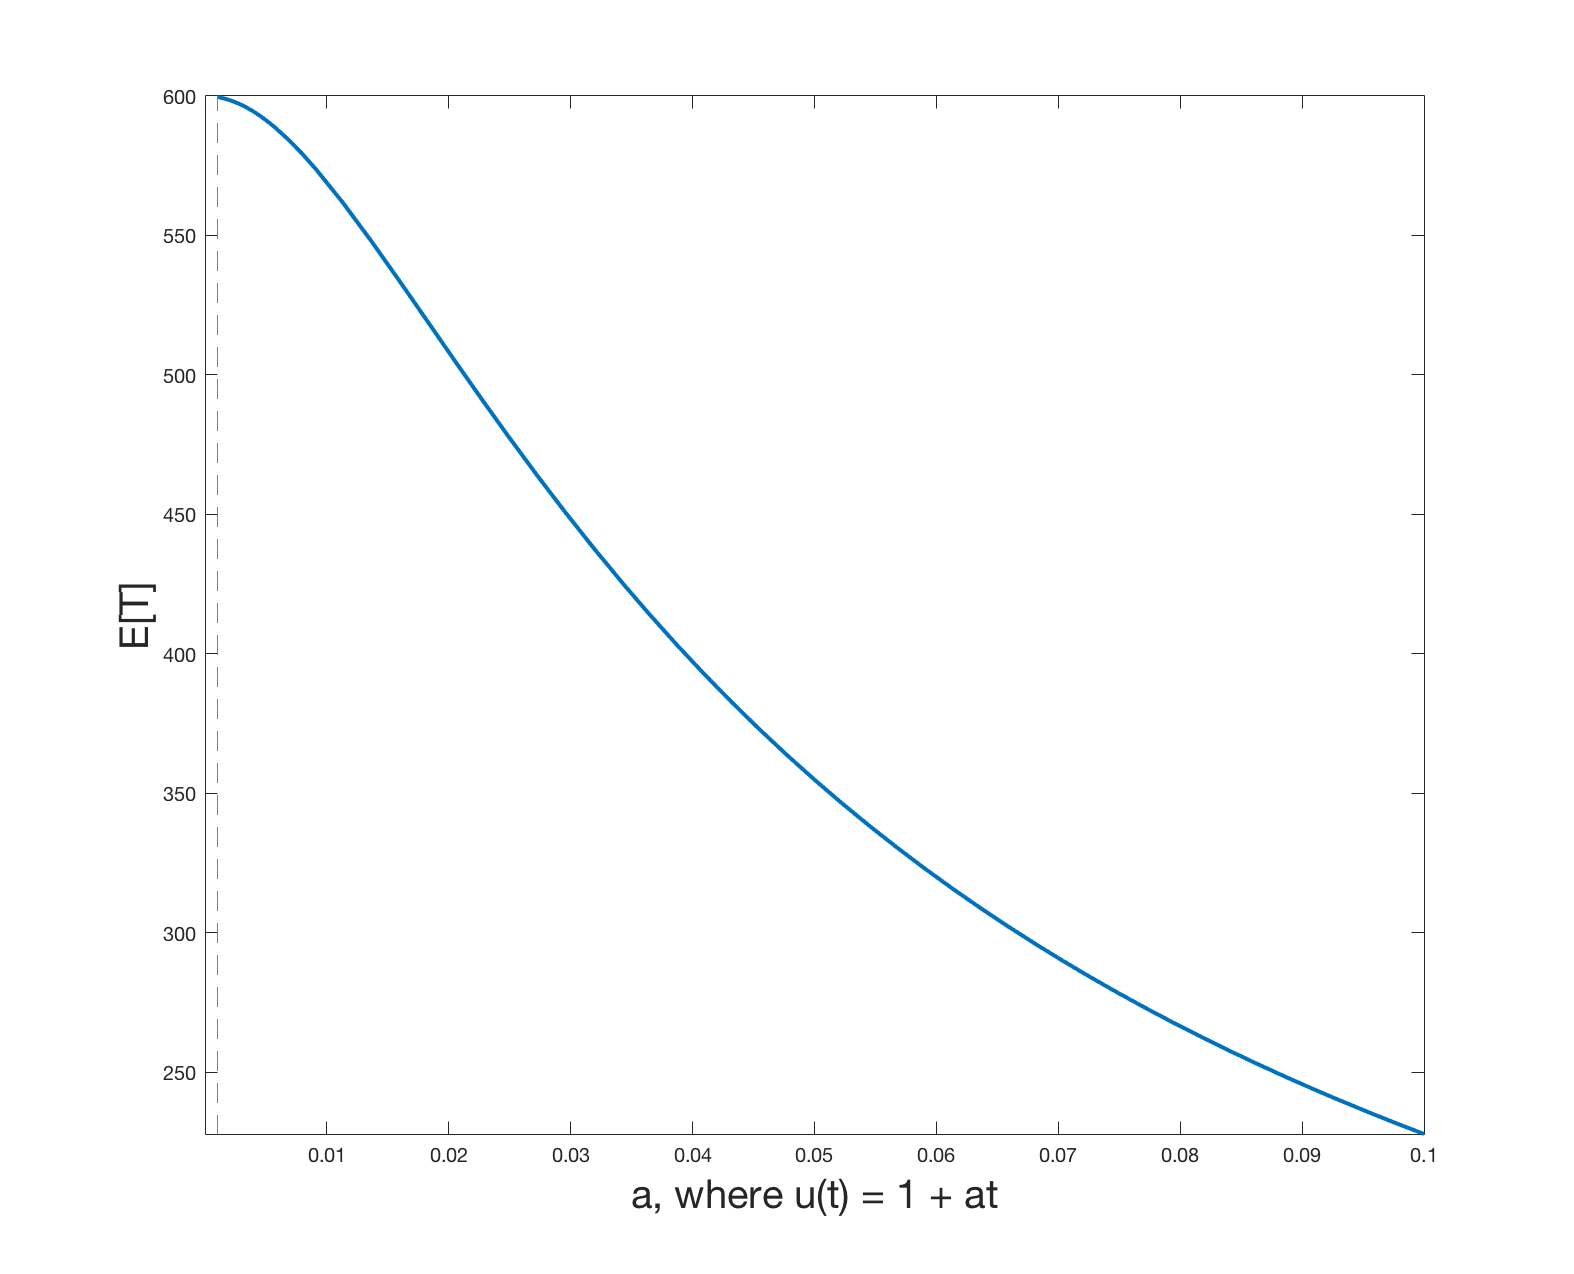
\includegraphics[width=\textwidth]{./images01/bitcoin-H-increasing.png}
%\caption{$\mathbf{E}[T]$ when H increases linearly with $u(t) = 1 + at$.\label{fig-bitcoin-H-increase}}
%\end{figure}


\section{Attack in the Bitcoin network}
% Ataque submarino
% Probabilidade de "correr por fora"

There are many possible ways to attack the Bitcoin \citep{karame2012two, heilman2015eclipse, bahack2013theoretical, bonneau2016buy, neudecker2015simulation}. In this section, we are interested in a particular attack: the double spending attack.

In the double spending attack, the attacker's send some funds to the victim, let's say a merchant. They wait for $k$ confirmations of the transaction, and the victim delivers the good or the service to the attacker. Then, the attacker mine enough blocks with a conflicting transaction, double spending the funds which was sent to the victim. If the attacker is successful, the original transaction will be \textit{erased} and the victim will be left with no funds at all. In order to be successful, the attacker must propagate more blocks than the network in the same period, propagating a chain longer than the main chain. Hence, we would like to understand what the odds are that the attacker will be successful. This attack was originally discussed by \citet{nakamoto2008bitcoin}.

In order to maximize their odds, the attacker must start to mine the new blocks as soon as they send the funds to the victim. In this moment, it starts to mine in the head of the blockchain, just like the rest of the network. So, in the beginning, the attacker and the network are in exactly the same point.

Let $\beta H$ be the hash rate of the attackers, and $\gamma H$ be the network's hash rate without the attackers. Thus, when $H \rightarrow +\infty$, we already know that $T_{\text{attackers}}$ and $T_{\text{network}}$ follow exponential distributions with parameters $\lambda_{\text{attacker}} = \frac{\beta}{\eta}$ and $\lambda_{\text{network}} = \frac{\gamma}{\eta}$, respectively.

As \cite{nakamoto2008bitcoin} has done, we will also model the attack using the Gambler's Ruin. In this game, a gambler wins \$1 at each round, with probability $p$, and loses \$1, with probability $1-p$. The rounds are independent. The gambler starts with \$$k$ plays continuously until he either accumulates a target amount of \$$m$, or loses all his money. Let $\rho = \frac{1-p}{p}$, then the probability of losing his fortune is:

$$
\mathbf{P}(\text{losing his fortune}) =
\begin{cases}
	\frac{\rho^k - \rho^m}{1-\rho^m} \text{, if $\rho \ne 1$,} \\
	\frac{m-k}{m} \text{, if $\rho = 1$.}
\end{cases}
$$

When $m \rightarrow +\infty$,

$$
\mathbf{P}(\text{losing his fortune}) =
\begin{cases}
	\rho^k \text{, if $\rho < 1$,} \\
	1 \text{, if $\rho \geq 1$.}
\end{cases}
$$

% TODO Expected time to absorption.

The gambler winning \$1 is the same as the network finding a new block, the gambler losing \$1 is the same as the attacker finding a new block. The initial \$$k$ is the same as the number of blocks the attacker is behind the network. Thus, the gambler loses his fortune is the same as the attacker successfully finds $k$ or more blocks than the network, i.e., losing his fortune means that the attack was successful.

In our case, $p = \frac{\lambda_{\text{network}}}{\lambda_{\text{network}} + \lambda_{\text{attacker}}} = \frac{\gamma}{\beta + \gamma}$, thus $\rho = \frac{\beta}{\gamma}$. Hence, $\rho < 1 \Leftrightarrow \beta < \gamma$.

Suppose that the attacker is mining with the network. Suddently, he stops mining with the network and starts attacking, i.e., starts to mine in another chain. In this scenario, since the attacker's hash rate is not mining with the network anymore, $\gamma = 1 - \beta$. Thus, $\beta < \gamma \Rightarrow \beta < 0.5 \Leftrightarrow \rho < 1$. Here comes the conclusion that, if the attacker has 50\% or more of the network's hash rate, then his attack will be certainly successful. We got exactly the same equations and conclusions as \cite{nakamoto2008bitcoin}.

But this scenario seems not to be the optimal attack, because the attacker has waited $k$ confirmations before starting the attack. A better approach would be to start attacking just after propagating the transaction. In this case, our previous model is not good, because even if the attacker have found more blocks than the network, he cannot propagate those blocks before the network has found $k$ confirmations. So, we have to model the probabilities before the network has found the $k$ block. Then, if the attacker has more blocks than the network, he has successfully attacked. Otherwise, we return to the previous model, in which the attacker must still find more blocks.

\begin{theorem}
	Assuming that the attacker starts the attack just after publishing the transaction, the probability of the attacker has already found exactly $s$ blocks while it waits the network to find $k$ blocks is $\mathbf{P}(S = s) = \binom{k+s-1}{s} (1-p)^s p^k.$
\end{theorem}
\begin{proof}
The attacker must find exactly $s$ blocks while the network must find exactly $k$ blocks. It is as they would be walking the grid from the point $(0, 0)$ to $(s, k)$, where it is only allowed to go up or right, like in Figure \ref{figure:bitcoin-attack-paths}. When the attacker finds a block, it would be a movement to the right. When the network finds a block, it would be an upward movement. No matter the order which the blocks are found, all the paths occur with probability $(1-p)^s p^k$.

The walking ends when $(\cdot, k$) is reached, i.e., when the network finds $k$ blocks, regardless of how many blocks the attacker has found -- i.e., it is not allowed to walk above the line $(\cdot, k)$. Thus, the number of paths between $(0, 0)$ and $(s, k)$ moving only upward or to the right, without going into the line $(\cdot, k)$ is exactly the number of paths between $(0, 0)$ and $(s, k-1)$, which is equal to the number of permutations of the sequence $(u, u, \dots, u, r, r, \dots, r)$ in which there are $s$ movements to the right ($r$) and $k-1$ upward movements ($u$). This number of permutations is $\frac{(k-1+s)!}{s!(k-1)!} = \binom{(k-1)+(s)}{s}$ because there are $s$ repetitions of the element $r$ and $k-1$ repetitions of the element $u$.

Finally, the probability is $\binom{k+s-1}{s} (1-p)^{s} p^{k}$.

\begin{figure}[ht]
  \centering
  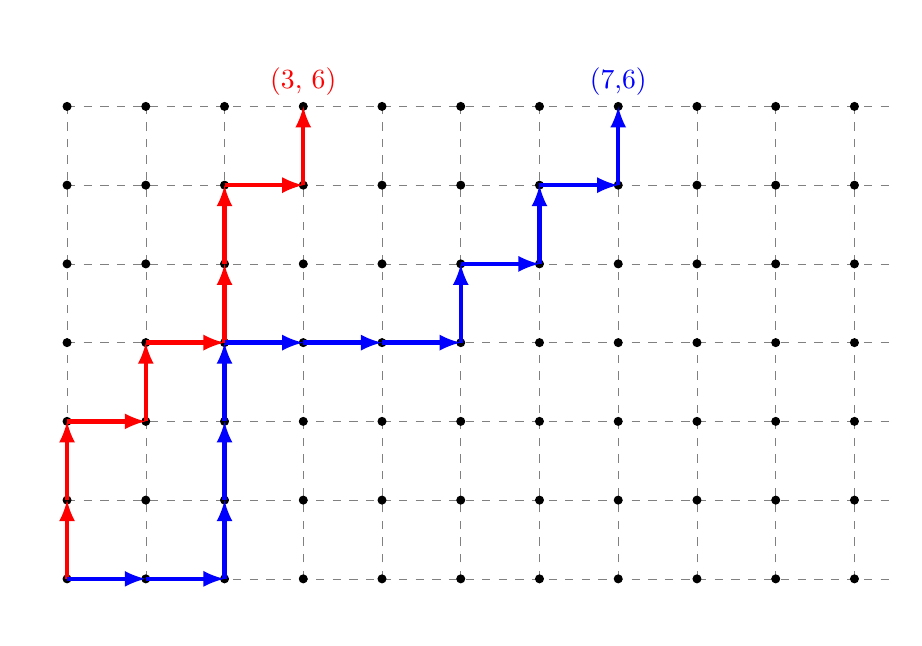
\begin{tikzpicture}
    \coordinate (Origin)   at (0,0);
    \coordinate (XAxisMin) at (-1,0);
    \coordinate (XAxisMax) at (5,0);
    \coordinate (YAxisMin) at (0,-1);
    \coordinate (YAxisMax) at (0,5);
    %\draw [thin, gray,-latex] (XAxisMin) -- (XAxisMax);% Draw x axis
    %\draw [thin, gray,-latex] (YAxisMin) -- (YAxisMax);% Draw y axis

    \clip (-0.5,-0.5) rectangle (10.5cm,7cm); % Clips the picture...
    %\pgftransformcm{1}{0}{0}{1}{\pgfpoint{0cm}{0cm}}
          % This is actually the transformation matrix entries that
          % gives the slanted unit vectors. You might check it on
           % MATLAB etc. . I got it by guessing.
    \draw[style=help lines,dashed] (0,0) grid[step=1cm] (14,6);
          % Draws a grid in the new coordinates.
          %\filldraw[fill=gray, fill opacity=0.3, draw=black] (0,0) rectangle (2,2);
              % Puts the shaded rectangle
    \foreach \x in {0,1,...,10}{% Two indices running over each
      \foreach \y in {0,1,...,6}{% node on the grid we have drawn
        \node[draw,circle,inner sep=1pt,fill] at (\x,\y) {};
            % Places a dot at those points
      }
    }

    \draw [ultra thick,-latex,red] (0,0) -- (0,1) node [midway, left] {};
    \draw [ultra thick,-latex,red] (0,1) -- (0,2) node [midway, left] {};
    \draw [ultra thick,-latex,red] (0,2) -- (1,2) node [midway, above] {};
    \draw [ultra thick,-latex,red] (1,2) -- (1,3) node [midway, right] {};
    \draw [ultra thick,-latex,red] (1,3) -- (2,3) node [midway, right] {};
    \draw [ultra thick,-latex,red] (2,3) -- (2,4) node [midway, right] {};
    \draw [ultra thick,-latex,red] (2,4) -- (2,5) node [midway, right] {};
    \draw [ultra thick,-latex,red] (2,5) -- (3,5) node [midway, right] {};
	\draw [ultra thick,-latex,red] (3,5) -- (3,6) node [above] {(3, 6)};

    \draw [ultra thick,-latex,blue] (0,0) -- (1,0) node [midway, left] {};
    \draw [ultra thick,-latex,blue] (1,0) -- (2,0) node [midway, left] {};
    \draw [ultra thick,-latex,blue] (2,0) -- (2,1) node [midway, left] {};
    \draw [ultra thick,-latex,blue] (2,1) -- (2,2) node [midway, left] {};
    \draw [ultra thick,-latex,blue] (2,2) -- (2,3) node [midway, left] {};
    \draw [ultra thick,-latex,blue] (2,3) -- (3,3) node [midway, left] {};
    \draw [ultra thick,-latex,blue] (3,3) -- (4,3) node [midway, left] {};
    \draw [ultra thick,-latex,blue] (4,3) -- (5,3) node [midway, left] {};
    \draw [ultra thick,-latex,blue] (5,3) -- (5,4) node [midway, left] {};
    \draw [ultra thick,-latex,blue] (5,4) -- (6,4) node [midway, left] {};
    \draw [ultra thick,-latex,blue] (6,4) -- (6,5) node [midway, left] {};
    \draw [ultra thick,-latex,blue] (6,5) -- (7,5) node [midway, left] {};
	\draw [ultra thick,-latex,blue] (7,5) -- (7,6) node [above] {(7,6)};
  \end{tikzpicture}
  \caption{Both the attacker and the network are mining. Each step up is a new block found by the network with probability $p$. Each step right is a new block found by the attacker with probability $1-p$. It ends when the network finds $k$ blocks --- in this example, $k=6$. The red path has probability $p^6 (1-p)^3$, while the blue path has probability $p^6 (1-p)^7$. Notice that the blue path is a successfull attack, because the attacker has found more blocks than the network. In the red path, the attacker still have to catch up 3 blocks to have a successful attack, which happens with probability $\rho^3$, if $p < 0.5$.}
  \label{figure:bitcoin-attack-paths}
\end{figure}
\end{proof}

Assuming that the attacker starts mining just after publishing the victim's transaction, the probability of the attacker will have found more than $k$ blocks while it waits the network to find $k$ blocks is $\mathbf{P}(S \geq k) = \sum_{s=k}^{\infty} \binom{k+s-1}{s} (1-p)^s p^k$.

\begin{theorem}
	$$\mathbf{P}(S \geq k) = 1 - \sum_{s=0}^{k-1} \binom{k+s-1}{s} (1-p)^s p^k.$$
\end{theorem}
\begin{proof}
	Let's use the following identity:
	$$\frac{1}{(1-z)^{a+1}} = \sum_{i=0}^{\infty} \binom{i+a}{i} z^i \text{, for $|z|<1$}$$

	Thus, replacing $z=1-p$, $i=s$, and $a=k-1$, we have:

	$$\frac{1}{p^{k}} = \sum_{s=0}^{\infty} \binom{s+k-1}{s} (1-p)^s$$
	$$1 = \sum_{s=0}^{\infty} \binom{s+k-1}{s} (1-p)^s p^k.$$

	Now, just split $\sum_{s=0}^{\infty} = \sum_{s=0}^{k-1} + \sum_{s=k}^{\infty}$ and it is done.
\end{proof}

Using this last theorem, we moved from an infinity sum to a finity sum.

\begin{theorem}
	Let $p = \frac{\gamma}{\beta + \gamma}$.
$$
\mathbf{P}(\text{successful attack}) =
\begin{cases}
%1 - \sum_{s=0}^{k-1} \binom{k+s-1}{s} (1-p)^s p^k \left(1 - \left( \frac{1-p}{p} \right)^{k-s} \right)
	1 - \sum_{s=0}^{k-1} \binom{k+s-1}{s} \left( (1-p)^s p^k - (1-p)^k p^s \right) \text{, $p \geq 0.5$} \\
	1 \text{, $p < 0.5$}.\\
\end{cases}
$$
\end{theorem}
\begin{proof}
$$
\mathbf{P}(\text{successful attack}) = \mathbf{P}(S \geq k) + \sum_{i=0}^{k-1} \mathbf{P}(s=i) \rho^{k-i}
$$
\end{proof}


For $k=6$, $p=0.9$, $\mathbf{P}(\text{successful attack}) = 0.0005914121600000266$.

For $k=6$, $p=0.7$, $\mathbf{P}(\text{successful attack}) = 0.15644958192000014$.

\begin{figure}[ht]
\centering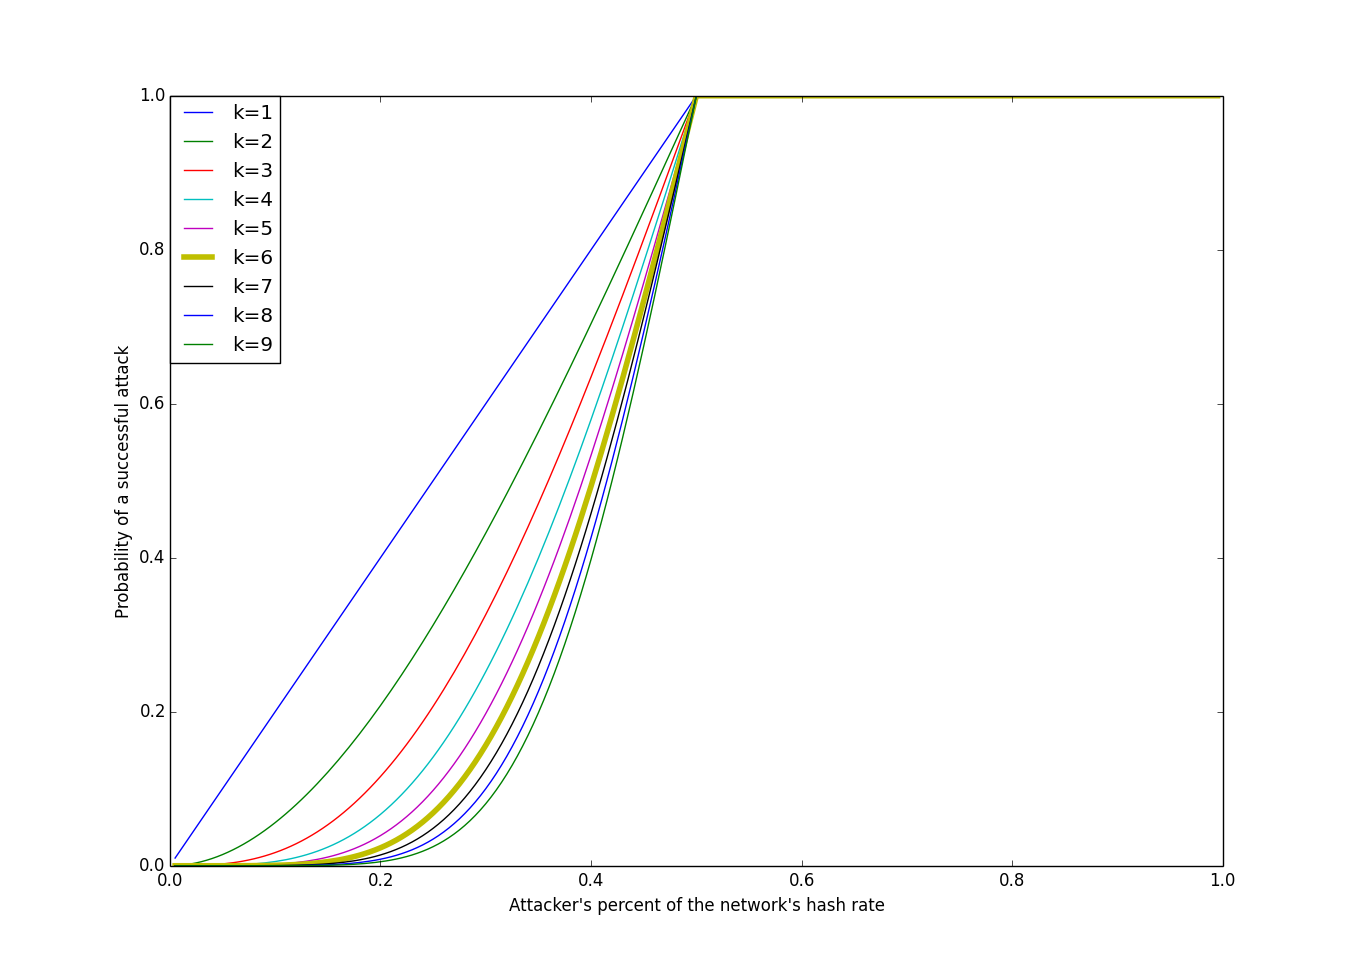
\includegraphics[width=\textwidth]{./images01/fig-bitcoin-attack.png}
\caption{Probability of a successful attack according to the network's hash rate of the attacker ($\beta$).\label{fig-bitcoin-attack}}
\end{figure}

% TODO Analyze when $k=2$ (for instance, Binance requires only two confirmations for deposits with less than $1,000$).

%The number of blocks found in a given time interval $\Delta t$ is given by the Poisson distribution. So, the number of blocks found by the attackers $N_{\text{attacker}}$ follows a Poisson distribution with parameter $\lambda_{\text{attacker}} \Delta t = \frac{\beta \Delta t}{600}$, and the number of blocks found by the network $N_{\text{network}}$ follows a Poission distribution with parameter $\lambda_{\text{network}} \Delta t = \frac{\gamma \Delta t}{600}$. We would like to calculate $\mathbf{P}(N_{\text{attackers}} - N_{\text{network}} \geq k)$.

%$\mathbf{P}(Y_{n+k}^{\text{attacker}} < Y_{n}^{\text{network}})$


\section{Confirmation time and network capacity}
% Tempo na fila para confirmar transação

Let's say that when a new transaction is propagated it is enqueued in the unconfirmed transaction queue. Then, when a new block is found, some of these transactions in the queue are confirmed. We are interested in some measures of the queue, like the expected time to confirm a transaction and the queue's length.

Let's assume that all transactions have exactly the same size $S$ and pay exactly the same fee. If the Bitcoin block's maximum size is $M$, there would be room for $s = \lfloor M/S \rfloor$ transactions in each block.

Using the results from \citet{bailey1954queueing}, we have found that $\pi_n = \frac{z_s-1}{z_s^{n+1}}$ is the probability of having $n$ unconfirmed transactions in the pool subjected to $s > m$, where $m=\frac{\lambda_{\text{TX}}}{\lambda_{\text{blocks}}}$ and $z_s$ is the single root of the polynomial $z^s(1+m(1-z))-1$ with $|z_s|>1$. In this case, the average size of the unconfirmed transaction pool is $\mathbf{E}(\pi) = \frac{1}{z_s - 1}$.

When $s > m$, the probabilities $\pi_n$ form a simple geometric series with common ratio smaller than one, which means the probabilities are exponentially decreasing. Since $\pi_n \rightarrow 0$ when $n \rightarrow \infty$, we may interpret it as a stable system, i.e., the unconfirmed transactions pool size is finite.

When $s \le m$, the system is unstable, which means the unconfirmed transactions pool size keeps growing towards infinity. In this case, the system is not capable of processing the demand for a long period of time.

Using the fact that $m=\frac{\lambda_{\text{TX}}}{\lambda_{\text{blocks}}}$ and $\lambda_{\text{blocks}} = 1/\eta$, the stability condition $s > m$ is reached when $\lambda_{\text{TX}} < s/\eta$.

In the Bitcoin's network, the average number of transactions per block is $s=2,250$, so, the system is stable when $\lambda_{\text{TX}} < 2,250/600 = 3.75$ tx/s. Therefore, $3.75$ is the maximum number of new transactions per second that the Bitcoin's network may handle. When $\lambda_{\text{TX}} > 3.75$ tx/s, the unconfirmed transaction pool starts to grow indefinitely.

When the system is stable, the average waiting time of a transaction to be confirmed is $\mathbf{E}(w) = \frac{1}{\lambda_{\text{TX}} (z_s-1)}$.

$m \ll s$ yields $z_s \rightarrow 1 + 1/m$. Thus, the average number of unconfirmed transactions $\mathbf{E}(\pi) \rightarrow m$ and the average waiting time $\mathbf{E}(w) \rightarrow \frac{1}{\lambda_{\text{blocks}}} = \eta = 600 \text{ seconds}$. In the Bitcoin's network, $m \ll s$ is reached when $\lambda_{\text{TX}} \ll 3.75$ tx/s. In other words, when the number of new transactions per second is way smaller than 3.75 tx/s, the average waiting time of a transaction to be confirmed is 600 seconds, which means, on average, all transactions will be confirmed in the next block.

But, $\lambda_{\text{TX}} \rightarrow s/\eta$ yields $z_s \rightarrow 1$. Hence, $\mathbf{E}(\pi) \rightarrow +\infty$, which means the system is going towards instability.

Therefore, we conclude that the Bitcoin's network capacity is $\lambda_{\text{blocks}} = s/\eta = s/600$ transactions per second, where $s$ is the average number of transactions per block.

For instance, in order to be a stable system and process 15 transactions per second, each block would have to confirm, on average, 9,000 transactions. Bitcoin's network is really far from this point.


%\section{Fork analysis}

% TODO BIP's and signaling bit --- see BIP 9 and BIP 135.

%When a disagreement between miners' rules happens, that is referred as either a hard-fork or a soft-fork. It is said to be a soft-fork when the rules are backward compatible, and a hard-fork when the rules are not backward compatible. In general, a hard-fork relaxes the constraints, while the latter hardens them.

%Suppose that the miners' are split in two groups, $G_1$ and $G_2$, with different rules. Let's say $H_1$ and $H_2$ are their hash rate, respectively. We have two different scenarios to analyze: (i) when neither of them accepts other's blocks; and (ii) when $G_2$ accepts $G_1$'s blocks, but not the other way around.

%Scenario (i) is easy to analyze, as the network would split and, after a while, both difficulties will be adjusted. Then, they will be just like two different Bitcoin networks.

%Scenario (ii) is more trick. As $G_2$ accepts $G_1$ blocks, their hashrate will matter. If $H_1 > H_2$, then $G_2$ will frequently skip their blockchain, because $G_1$'s blockchain will be longer most of the time. If $H_1 < H_2$, then $G_2$ may have its own blockchain after a while --- a true fork. But what would happen if $H_1$ keeps increasing and eventually gets larger than $H_2$? It if happens for sufficient time, the whole $G_2$'s blockchain may be discarded in order to move to $G_1$'s blockchain when $G_1$'s gets longer.

%\begin{theorem}
%	When $H_1 > H_2$, the
%\end{theorem}



%What would happen if, after a while, the groups agree again. How would the blockchain merge?
